%!TEX root = ../main.tex

\section{Вычислительный эксперимент}

Была написана программа, реализующая разностную схему \eqref{sch:all}.

Все предыдущие рассуждения были универсальны для плоского, цилиндрического и сферического случаев, насколько это возможно. Все три случая моделируются одной и той же программой, принимающей $k = \overline{0, 2}$ как параметр.

Зададим параметры модели:
$$\epsilon_0 = 0.2, \; \delta = 0.04, \; l = 1.0, \; \Gamma = 1.0, \; m = 0.5 \tpoint$$

Пусть $R = 5$. По виду графиков будет понятно, что для использованного набора параметров такое $R$ достаточно велико.

Выберем число ячеек $n = 300$ при $\alpha = 0$ и $n = 150$ иначе. Шаг по пространству~$h$, соответственно, равен $1/60 \approx 0.0167$ либо $1/30 \approx 0.0333$. При этом придется брать шаг по времени $\tau = 5 \cdot 10^{-7}$. Если шаг по времени кратно больше, то схема оказывается неустойчива и программа завершается с ошибкой переполнения (в данных возникает значение NaN). Как и ожидалось, $p$-лапласиан и билапласиан (особенно) требуют относительно малых шагов по времени.

Выбор начальных условий неважен. Пусть, например, значения $0$ и $1$ гладко соединяются ветвью синусоиды: $\avphi_i^0 = \sin[(h/2 + ih) \pi / 2], \; h/2 + ih < 1$; далее все значения равны $1$.

Будем останавливать расчет, когда вектор <<воздействия>> на систему достаточно мал, а именно:
$$\max\limits_{i = 0}^n \cfrac{\avphi_i^{j + 1} - \avphi_i^j}{m} < 10^{-9} \tpoint$$
Все конфигурации модели достигли названного условия не более чем через~$7.4$ единицы времени.

\begin{figure}[!tp]
	\centering
	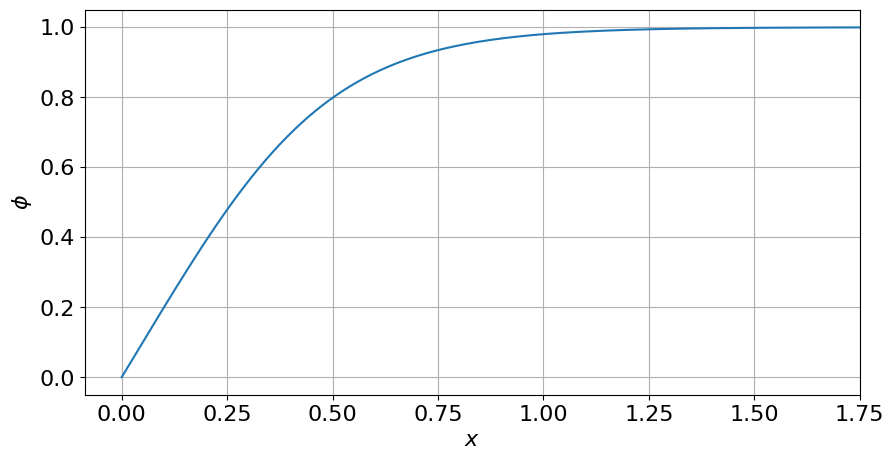
\includegraphics[width=0.83\textwidth]{figures/result_volumes.png}
	\vspace{-0.4cm}
	\caption{Решение $\phi$ в плоском случае при $\alpha = 0, \; \beta = 0$.}
	\label{fig:result_volumes}
	\vspace{0.5cm}

	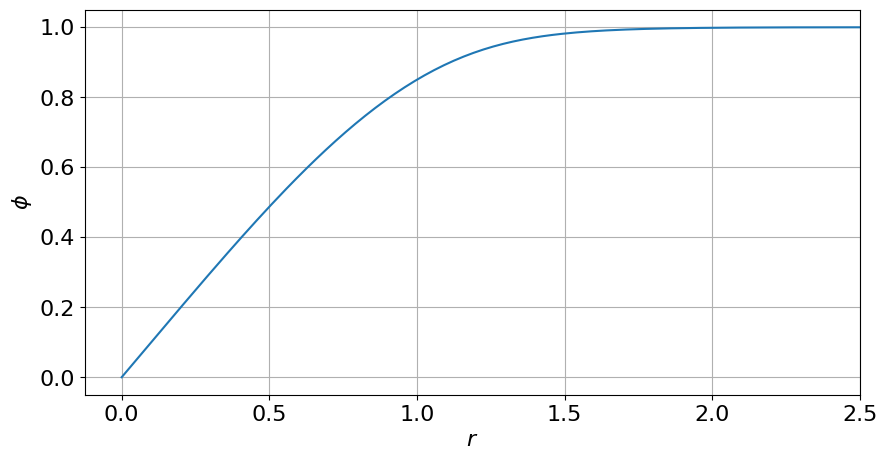
\includegraphics[width=0.83\textwidth]{figures/result_volumes_p.png}
	\vspace{-0.4cm}
	\caption{Решение $\phi$ в плоском случае при $\alpha = 0, \; \beta = 1$.}
	\label{fig:result_volumes_p}
	\vspace{0.5cm}
	
	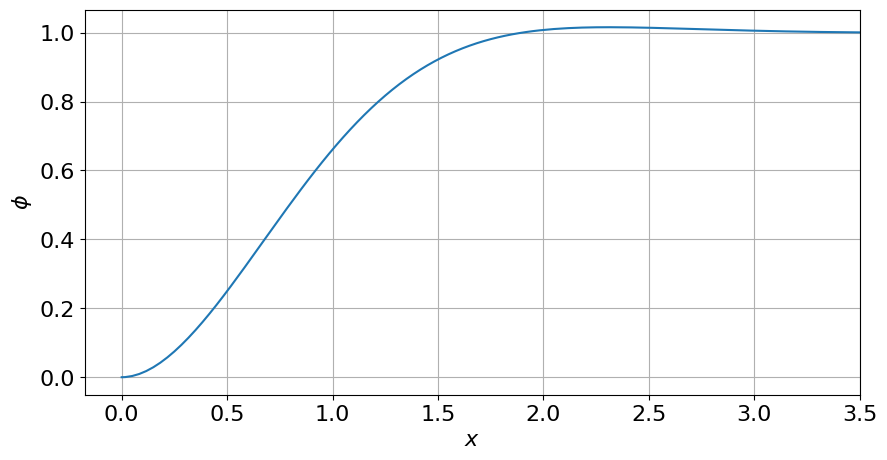
\includegraphics[width=0.83\textwidth]{figures/result_volumes_bi.png}
	\vspace{-0.4cm}
	\caption{Решение $\phi$ в плоском случае при $\alpha = 1, \; \beta = 0$.}
	\label{fig:result_volumes_bi}
\end{figure}

\begin{figure}[!tp]
	\centering
	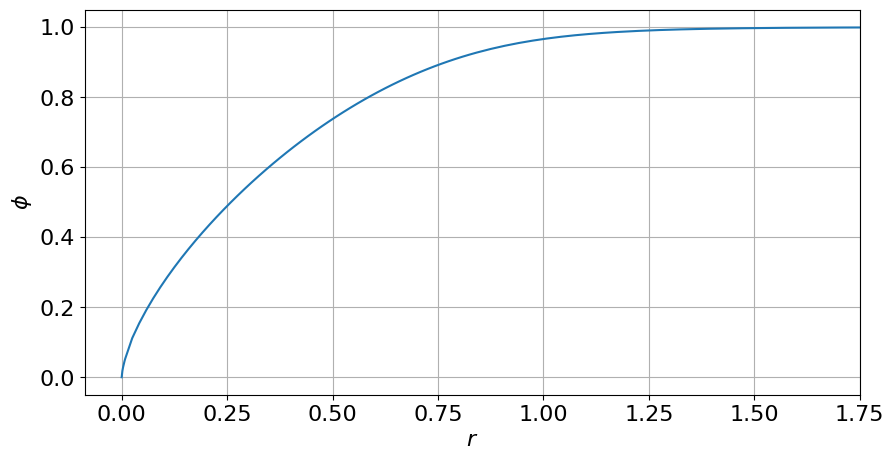
\includegraphics[width=0.83\textwidth]{figures/result_volumes_cyl_p.png}
	\vspace{-0.4cm}
	\caption{Решение $\phi$ в цилиндрическом случае при $\alpha = 0, \; \beta = 1$.}
	\label{fig:result_volumes_cyl_p}
	\vspace{0.5cm}

	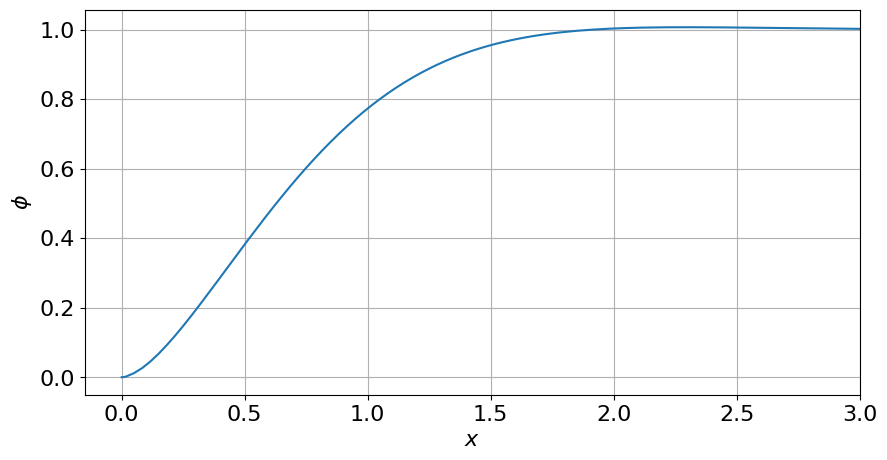
\includegraphics[width=0.83\textwidth]{figures/result_volumes_cyl_bi.png}
	\vspace{-0.4cm}
	\caption{Решение $\phi$ в цилиндрическом случае при $\alpha = 1, \; \beta = 0$.}
	\label{fig:result_volumes_cyl_bi}
	\vspace{0.5cm}
	
	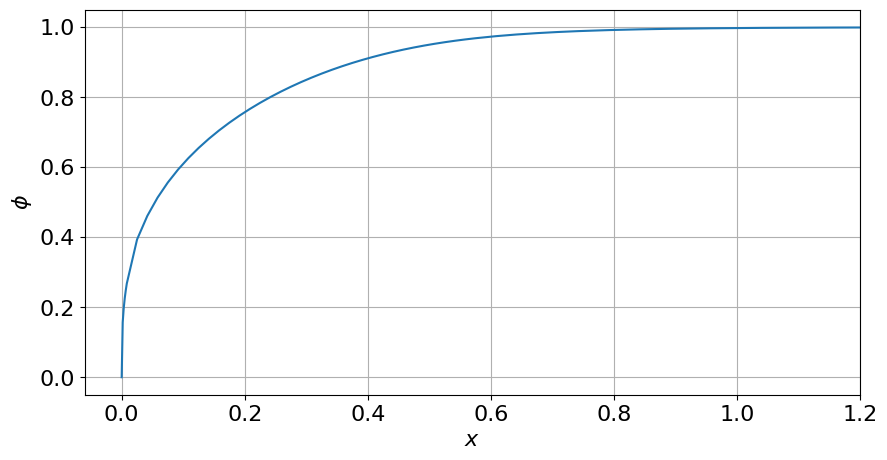
\includegraphics[width=0.83\textwidth]{figures/result_volumes_sph_p.png}
	\vspace{-0.4cm}
	\caption{Решение $\phi$ в сферическом случае при $\alpha = 0, \; \beta = 1$.}
	\label{fig:result_volumes_sph_p}
\end{figure}

Результаты вычислений изображены на рис. \ref{fig:result_volumes} и \ref{fig:result_volumes_p} (случай 1 из описания разностной схемы), рис. \ref{fig:result_volumes_bi} (случай 2), рис. \ref{fig:result_volumes_cyl_p} (случай 3), рис. \ref{fig:result_volumes_cyl_bi} (случай 4), рис.~\ref{fig:result_volumes_sph_p} (случай~5). Графики функций показаны до зримого момента выхода на примерно постоянное значение $1$, после чего они в действительности продолжаются до $R = 5$. Графики состоят из соединенных значений средних~$\avphi_i^j$, размещенных в серединах ячеек; вблизи~$0$ к ним добавлено несколько значений приближающей функции $g_{1/2}$, имеющей особенность в $0$, если того требует случай задачи.

Отметим, что если в уравнения входит билапласиан ($\alpha \neq 0$), то функция~$\phi$ может быть не монотонной и в некоторых точках превышать значение~$1$ (см.~рис.~\ref{fig:result_volumes_bi},~\ref{fig:result_volumes_cyl_bi}). В работе \cite{zipunova_higher_codimension} это было отмечено и указано, что монотонность~$\phi$ следует ожидать при достаточно малых $\alpha$.

Итак, эксперимент подтверждает, что, несмотря на некоторую громоздкость формулировок, предложенная модификация метода конечных объемов позволяет эффективно моделировать решение $\phi$, даже если на границе области оно имеет особенность.